\documentclass[11pt]{article}

% ---------- Packages (per course conventions) ----------
\usepackage[margin=1in]{geometry}
\usepackage{graphicx}
\usepackage{float}
\usepackage{booktabs}
\usepackage{siunitx}
\usepackage{amsmath}
\usepackage{amssymb}
\usepackage{tikz}
\usetikzlibrary{arrows.meta,calc}
\usepackage{tcolorbox}
\usepackage{enumitem}
\usepackage{xcolor}
\usepackage{hyperref}
\hypersetup{colorlinks=true, linkcolor=black, urlcolor=blue}

\setlength{\parindent}{0pt}
\setlength{\parskip}{\baselineskip}

% =========================================================
% EDIT THESE FOR EACH NEW ASSIGNMENT
% =========================================================
\newcommand{\assignmentNumber}{2}
\newcommand{\assignedDate}{}
\newcommand{\dueDate}{}
\newcommand{\numProblems}{8} % just for your own reference; add/remove \problempage calls below as needed

% ---------- Boxed-answer helper ----------
\newtcolorbox{finalanswer}{
    colback=white, colframe=black, boxrule=1pt,
    title=Answer, fonttitle=\bfseries, coltitle=black,
    colbacktitle=white
}

% ---------- Reusable problem scaffold ----------
% \problempage{Problem number}{Given/Find summary}{Sketch (tikzpicture etc.)}{Equations & Solution body}{Boxed final answer text}
\newcommand{\problempage}[5]{%
    \clearpage
    \section*{Problem #1}

    \textbf{Given / Find:} #2

    \vspace{0.3cm}
    \textbf{Sketch:}

    \begin{center}
    #3
    \end{center}

    \vspace{0.3cm}
    \textbf{Equations \& Solution:}

    \vspace{0.2cm}
    #4

    \begin{finalanswer}
        #5
    \end{finalanswer}
}

\begin{document}

% =========================================================
% COVERSHEET
% =========================================================
\begin{titlepage}
    \centering
    \vspace*{2cm}
    {\LARGE \bfseries ENGR 225: Mechanics 1} \\[0.3cm]
    {\Large Homework Coversheet} \\[0.3cm]
    {\large Assoc.\ Prof.\ Clayton Byers} \\[2cm]

    \begin{flushleft}
        \Large
        \textbf{NAME:} \underline{\hspace{2cm}Sean Balbale\hspace{2cm}} \\[1cm]
        \textbf{DATE:} \underline{\hspace{2cm}9/25/2026\hspace{2cm}} \\[1cm]
        \textbf{ASSIGNMENT:} \underline{\hspace{2cm}Homework 2\hspace{4cm}} \\[2cm]
    \end{flushleft}

    \large
    \textbf{Level of involvement of AI, LLMs, or related tools in the completion of this assignment:}

    \vspace{1cm}

    \begin{flushleft}
        \Large
        $\blacksquare$ \quad None \\[0.7cm]
        $\square$ \quad Minor \\[0.7cm]
        $\square$ \quad Major \\[0.7cm]
        $\square$ \quad Extensive \\[1.5cm]
    \end{flushleft}

    \normalsize
    \textit{Mark the box that applies (e.g., replace $\square$ with $\blacksquare$, or type an X beside it, before compiling/printing). Your disclosure does not affect your grade -- it keeps you accountable for the work you are doing.}

\end{titlepage}

% % =========================================================
% % HOMEWORK HEADER
% % =========================================================
% \section*{ENGR 225 -- Homework \assignmentNumber}
% \textbf{Assigned:} \assignedDate \hfill \textbf{Due:} \dueDate

% \vspace{0.3cm}
% \textit{Formatting per course guidelines: each problem on its own page, with problem summary, labeled sketch, governing equations, units carried throughout, results to 3 significant figures, and a clearly boxed final answer.}

% =========================================================
% PROBLEMS
% =========================================================

\problempage{1}{
A crane boom $OA$ (length 8 m) makes an angle $\theta=30^\circ$ with the horizontal. A towline force $P = 6\text{ kN}$ acts at $A$, directed toward a hook at $B$ on the ground, a horizontal distance $x$ from the point below $O$ ($O$ is 1 m above the ground). Find the placement $x$ that maximizes the moment of $P$ about $O$, and find that maximum moment.
}{
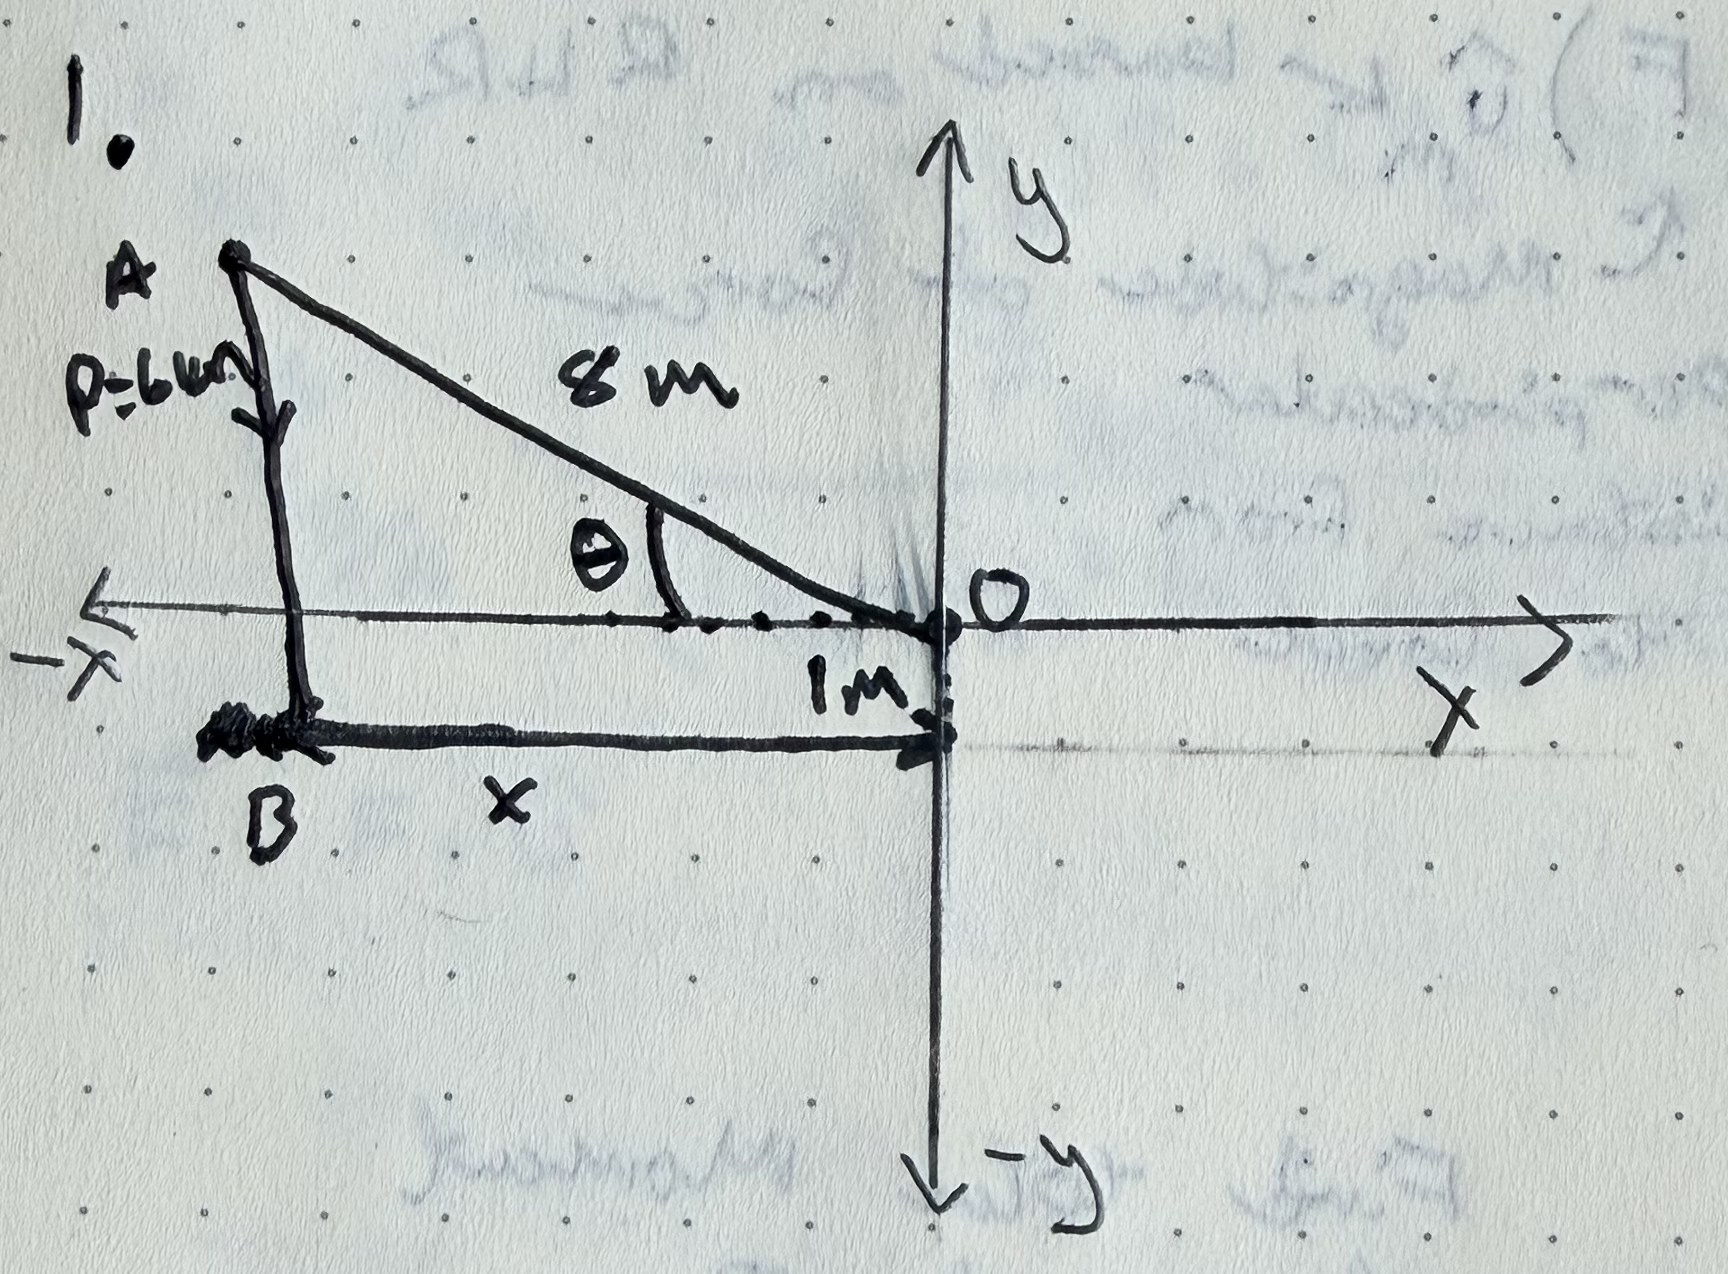
\includegraphics[width=0.7\textwidth,height=0.32\textheight,keepaspectratio]{photos/IMG_5527.jpg}
}{
Since $A$ and $O$ are fixed, the moment of a fixed-magnitude $P$ applied at $A$ is largest when the line of action $AB$ is \emph{perpendicular} to $OA$:
\[
M_{\max} = P\,(OA)
\]
Place $O$ at the origin, $x$ pointing left (toward $B$) and $y$ up:
\[
\vec{r}_{OA} = (8\cos30^\circ,\ 8\sin30^\circ) = (6.928,\ 4.000)\text{ m}, \qquad
\vec{r}_{AB} = (x-6.928,\ -1-4.000)
\]
Perpendicularity requires $\vec r_{OA}\cdot \vec r_{AB}=0$:
\[
6.928(x-6.928) + 4.000(-5.000) = 0
\]

\textbf{Solve:}
\[
6.928x = 6.928^2 + 20.0 = 48.0+20.0 = 68.0 \ \Rightarrow\ x = \frac{68.0}{6.928} = 9.81\text{ m}
\]
\[
M_{\max}= P\,(OA) = (6\text{ kN})(8\text{ m}) = 48.0\text{ kN}\cdot\text{m}
\]
}{
$x = 9.81\text{ m}$, \qquad $M = 48.0\text{ kN}\cdot\text{m}$
}

\problempage{2}{
A tower crane has a jib $BD$ (1.5 Mg, mass center $G_1$, 9.5 m right of the tower) carrying a 2 Mg load (12.5 m right of tower), and a counter-jib $BC$ (0.5 Mg, mass center $G_2$, 4 m left of tower) with counterweight $C$ (mass center $G_3$, 7.5 m left of tower). Find the counterweight mass $m$ so the net moment of all these weights about the base $A$ is zero.
}{
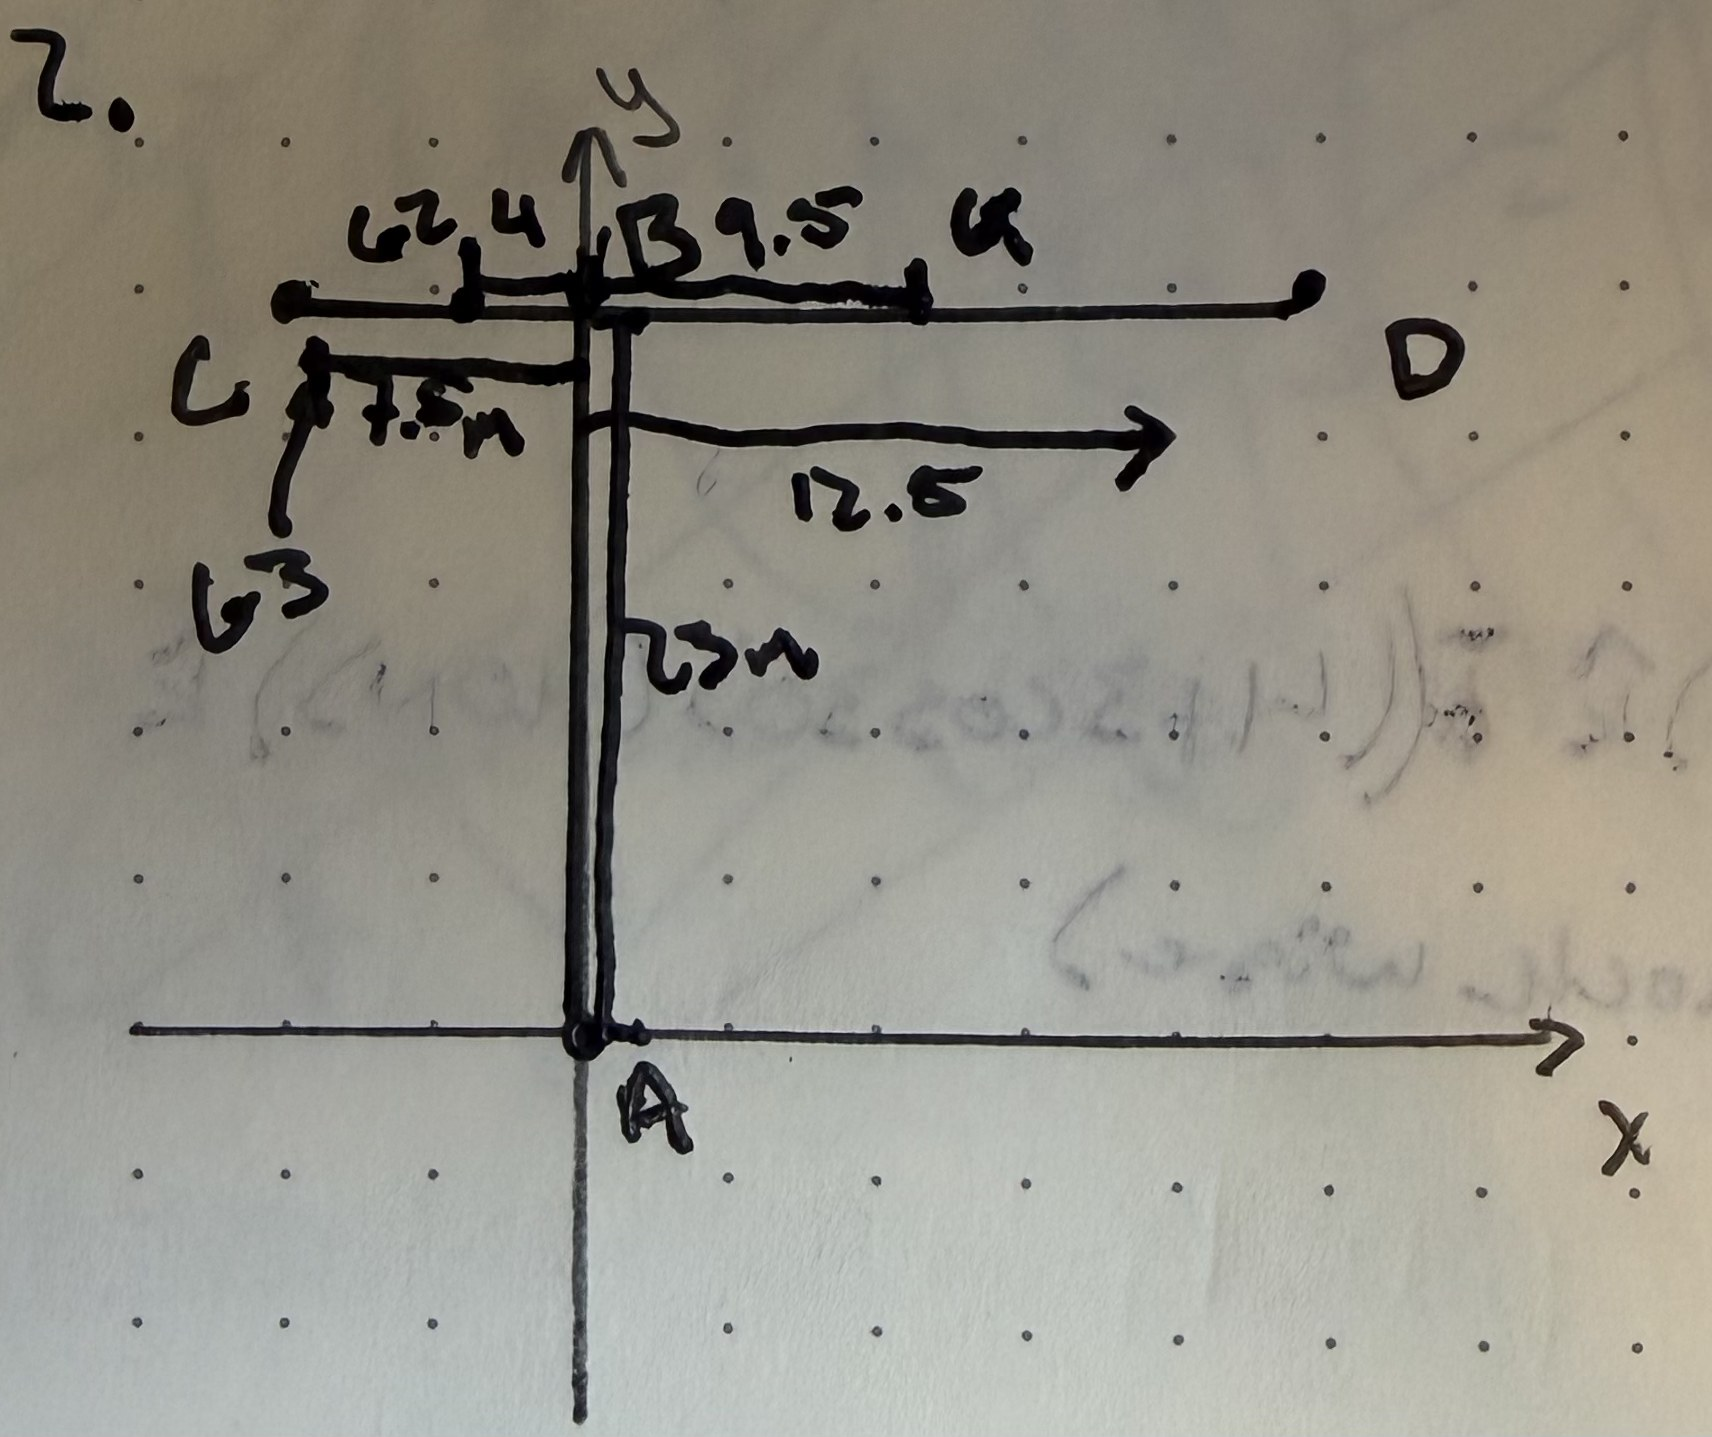
\includegraphics[width=0.7\textwidth,height=0.32\textheight,keepaspectratio]{photos/IMG_5528.jpg}
}{

\[
\sum M_{A}=0:\qquad (0.5\text{ Mg})(4\text{ m}) + m(7.5\text{ m}) = (1.5\text{ Mg})(9.5\text{ m}) + (2\text{ Mg})(12.5\text{ m})
\]

\textbf{Solve:}
\[
2.0 + 7.5\,m = 14.25 + 25.0 = 39.25
\]
\[
m = \frac{39.25-2.0}{7.5} = \frac{37.25}{7.5} = 4.97\text{ Mg}
\]
}{
$m = 4.97\text{ Mg}$
}

\problempage{3}{
$\vec F = 6\hat\imath+8\hat\jmath+10\hat k\ \text{N}$ produces a moment $\vec M_O = -14\hat\imath+8\hat\jmath+2\hat k\ \text{N}\cdot\text{m}$ about $O$. The line of action passes through a point with $x=1$ m. Find $y,z$ of that point, and the perpendicular distance $d$ from $O$ to the line of action.
}{
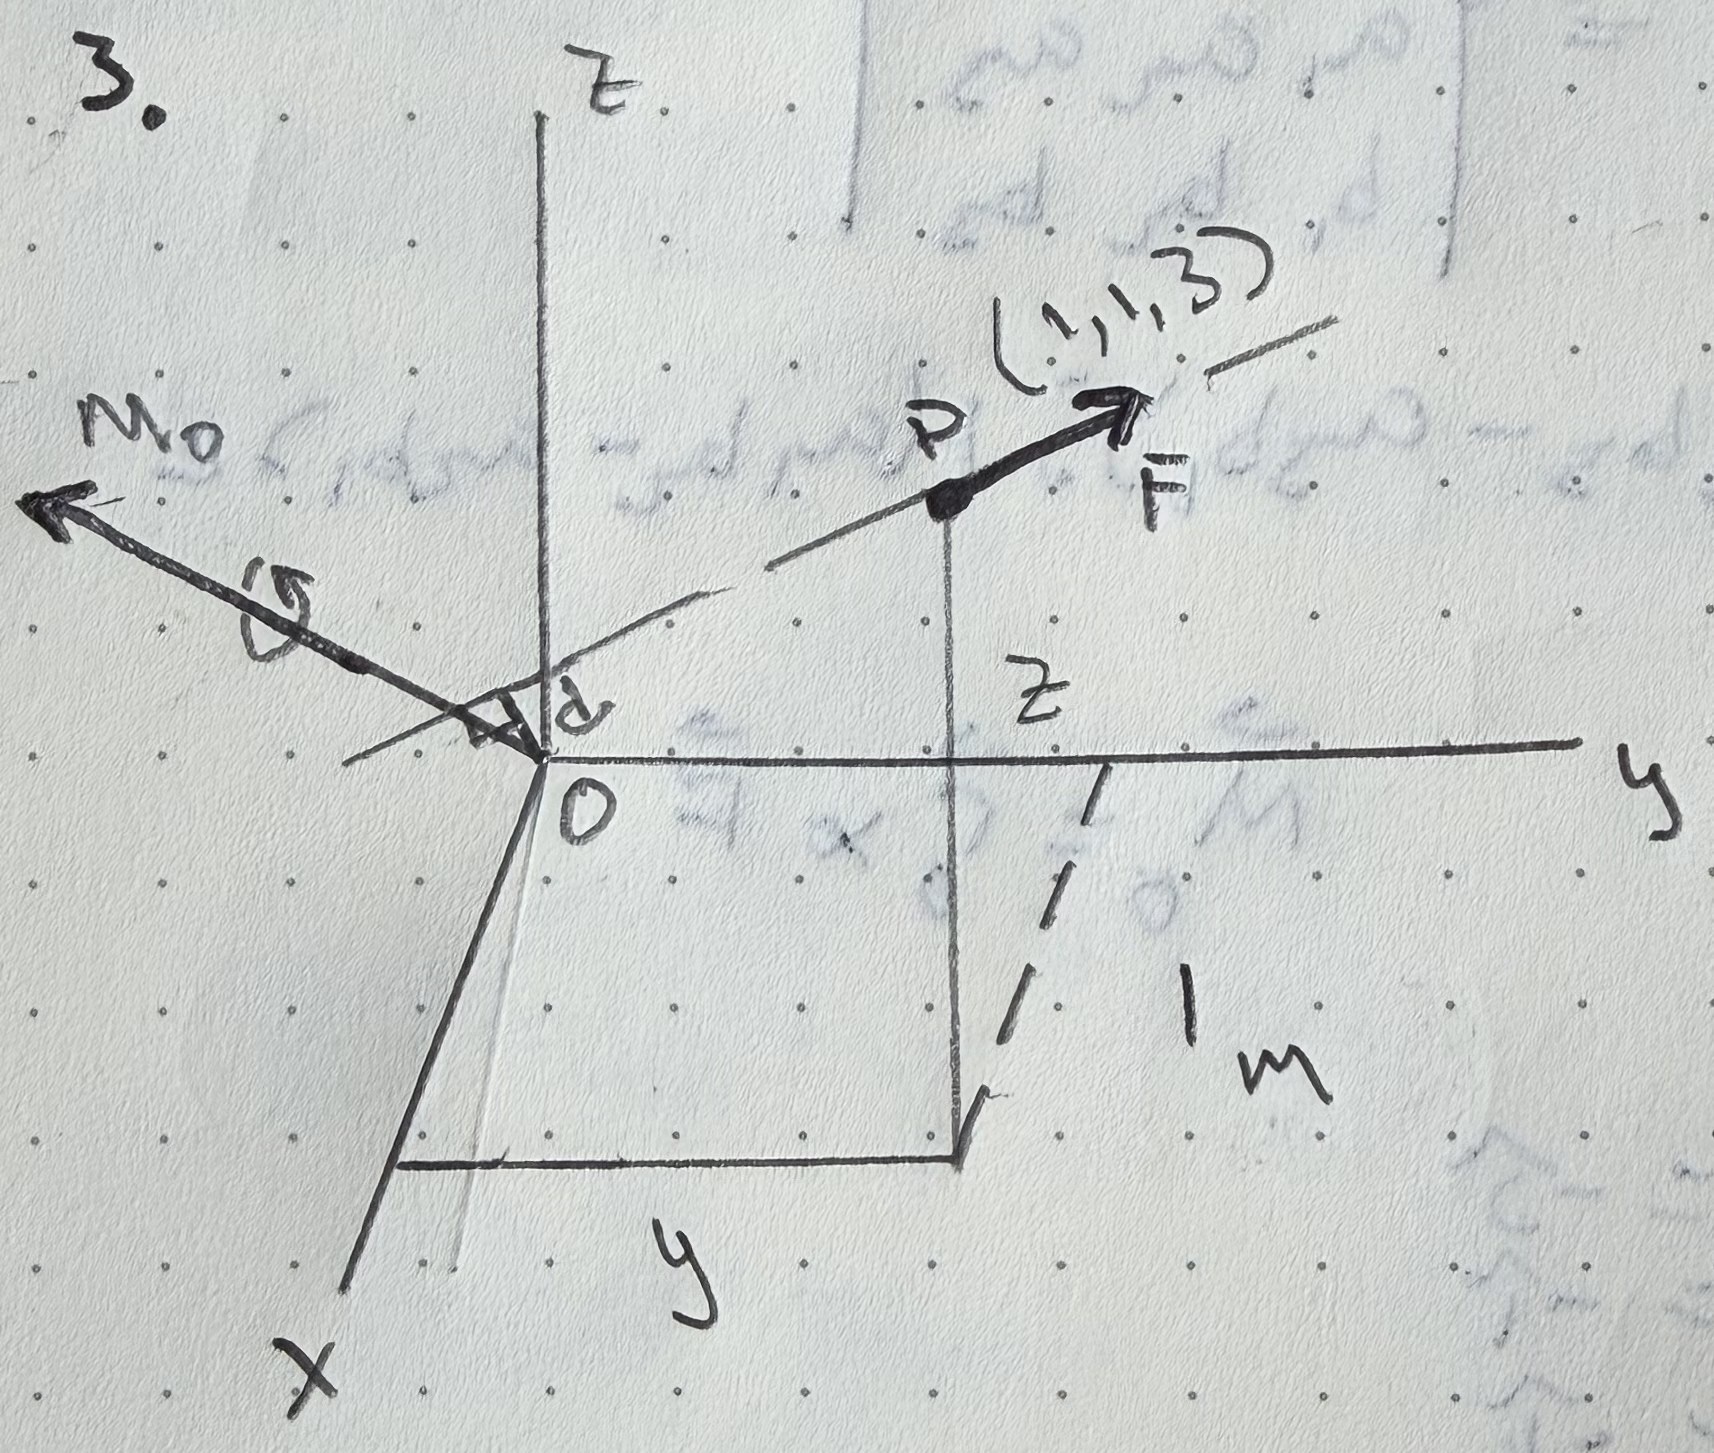
\includegraphics[width=0.7\textwidth,height=0.32\textheight,keepaspectratio]{photos/IMG_5529.jpg}
}{
The point lies at $\vec r = x\hat\imath+y\hat\jmath+z\hat k$ with $\vec M_O = \vec r\times \vec F$:
\[
\vec r\times\vec F=(10y-8z)\hat\imath-(10x-6z)\hat\jmath+(8x-6y)\hat k
\]
Matching components to $\vec M_O=(-14,8,2)$ with $x=1$:
\[
10y-8z=-14, \qquad -(10(1)-6z)=8, \qquad 8(1)-6y=2
\]

\textbf{Solve:} From the $\hat\jmath$-equation: $-10+6z=8\Rightarrow z=3.00$ m.
From the $\hat k$-equation: $8-6y=2\Rightarrow y=1.00$ m (check $\hat\imath$: $10(1)-8(3)=-14$ \checkmark).

For the perpendicular distance, since $|\vec M_O| = |\vec F|\,d$:
\[
d=\frac{|\vec M_O|}{|\vec F|}=\frac{\sqrt{14^2+8^2+2^2}}{\sqrt{6^2+8^2+10^2}}=\frac{\sqrt{264}}{\sqrt{200}} = \frac{2\sqrt{66}}{10\sqrt{2}} = \frac{\sqrt{33}}{5} \approx 1.15\text{ m}
\]
}{
$\vec r = 1\hat\imath+1\hat\jmath+3\hat k$ m \quad ($y=1.00$ m, $z=3.00$ m), \qquad $d = 1.15$ m
}

\problempage{4}{
A tripod has base points $B,C,A$ and apex $D$, with $\vec F = 50\hat\imath-20\hat\jmath-80\hat k\ \text{N}$ applied at $D$. Using the given dimensions, $A=(0,2,0)$ m, $B=(3.5,2.5,0)$ m, $C=(2,0,0)$ m, and $D=(2.5,2,4)$ m. Find the magnitude of the moment of $\vec F$ about line $CA$.
}{
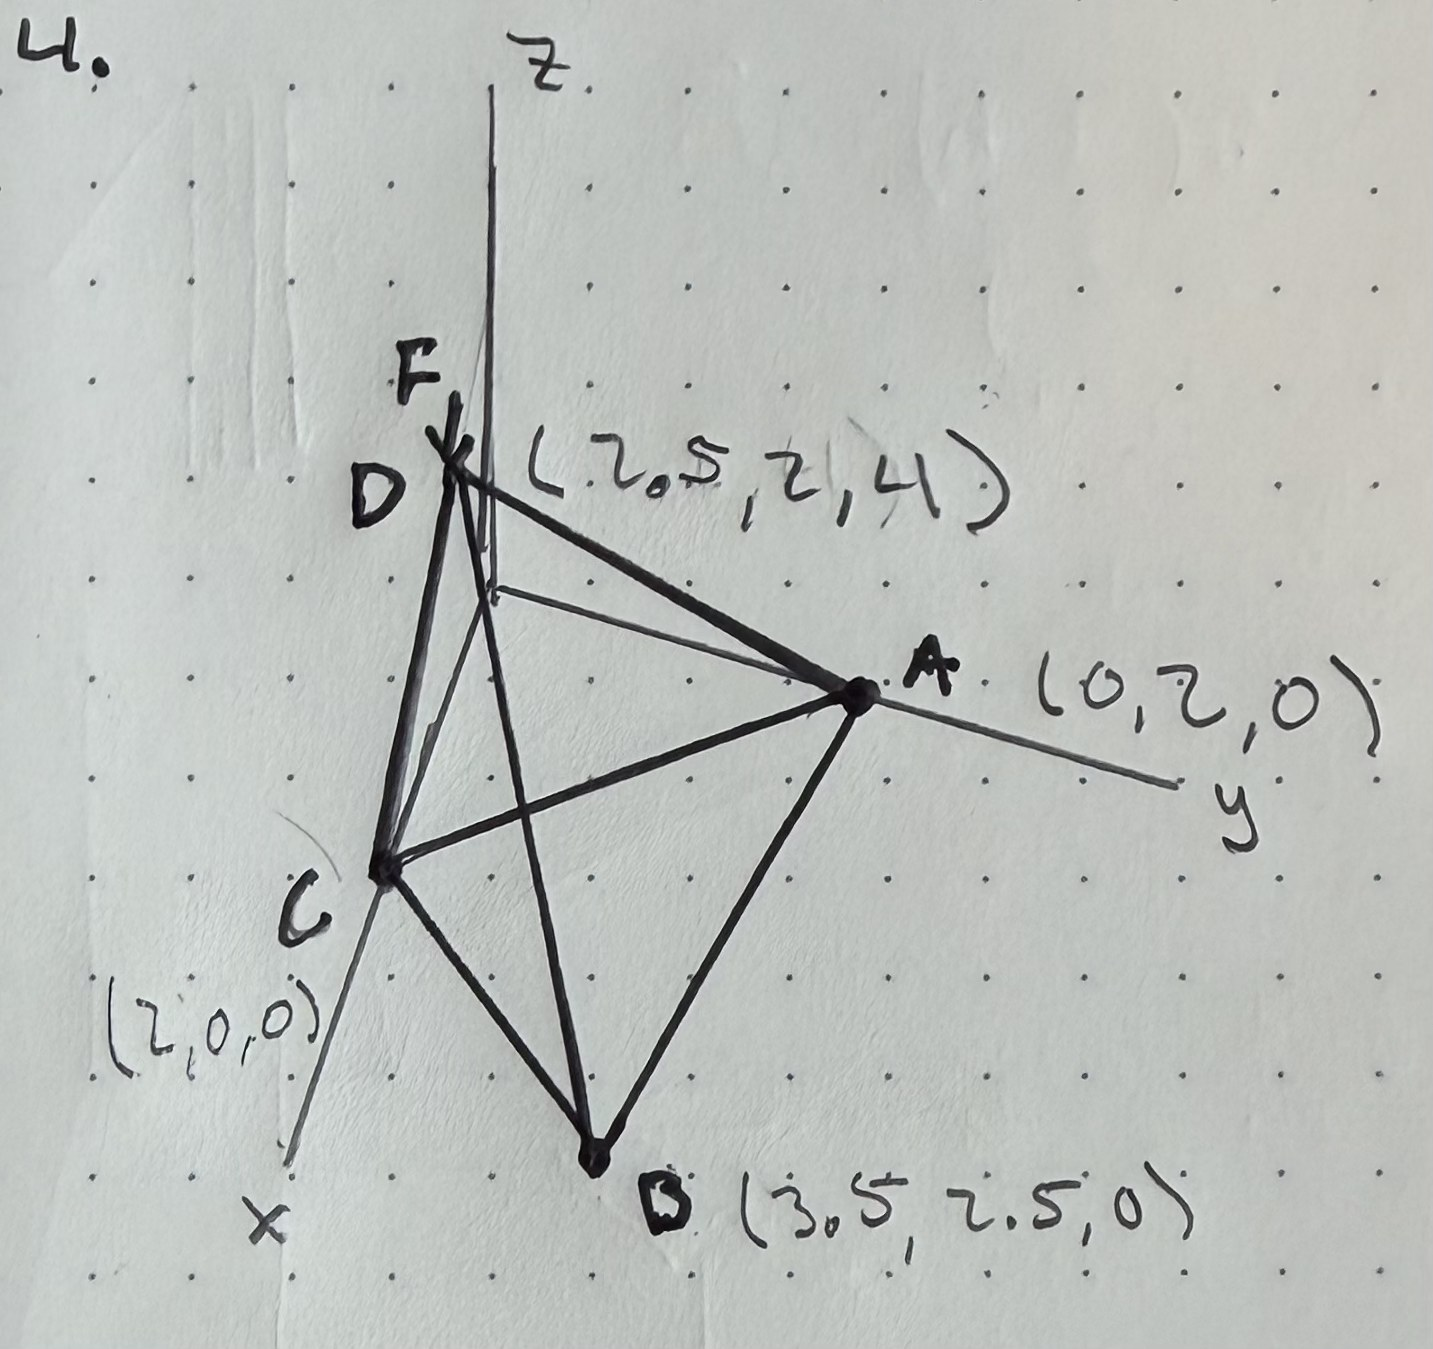
\includegraphics[width=0.7\textwidth,height=0.32\textheight,keepaspectratio]{photos/IMG_5541.jpg}
}{
Compute the moment of $\vec F$ about point $A$, then project onto the unit vector along $CA$:
\[
\vec r_{AD} = \vec r_D-\vec r_A, \qquad \vec M_A = \vec r_{AD}\times \vec F, \qquad
\hat u_{CA}=\frac{\vec r_A-\vec r_C}{|\vec r_A-\vec r_C|}, \qquad M_{CA}=\hat u_{CA}\cdot \vec M_A
\]

\textbf{Solve:}
\[
\vec r_{AD} = (2.5,\,0,\,4.0)\text{ m}
\]
\[
\vec M_A = \vec r_{AD}\times \vec F =
\begin{vmatrix}\hat\imath&\hat\jmath&\hat k\\ 2.5&0&4.0\\ 50&-20&-80\end{vmatrix}
= (80)\hat\imath+(400)\hat\jmath+(-50)\hat k\ \text{N}\cdot\text{m}
\]
\[
\hat u_{CA}=\frac{(-2,\,2,\,0)}{2.828}=(-0.7071,\,0.7071,\,0)
\]
\[
M_{CA}=\hat u_{CA}\cdot\vec M_A = (-0.7071)(80)+(0.7071)(400)+0 = 226.3\ \text{N}\cdot\text{m}
\]
}{
$M_{CA} = 226\ \text{N}\cdot\text{m}$
}

\problempage{5}{
A symmetric crank pivoted at $O$ has two straight arms at $45^\circ$ to the horizontal. On each arm a rod is pinned at $4$ in from $O$ (carrying $F$ / $-F$, each $30^\circ$ from vertical) and at $9$ in from $O$ (carrying the $150$ lb forces, each $30^\circ$ from horizontal). Find $F$ so the net couple moment on the crank is zero.
}{
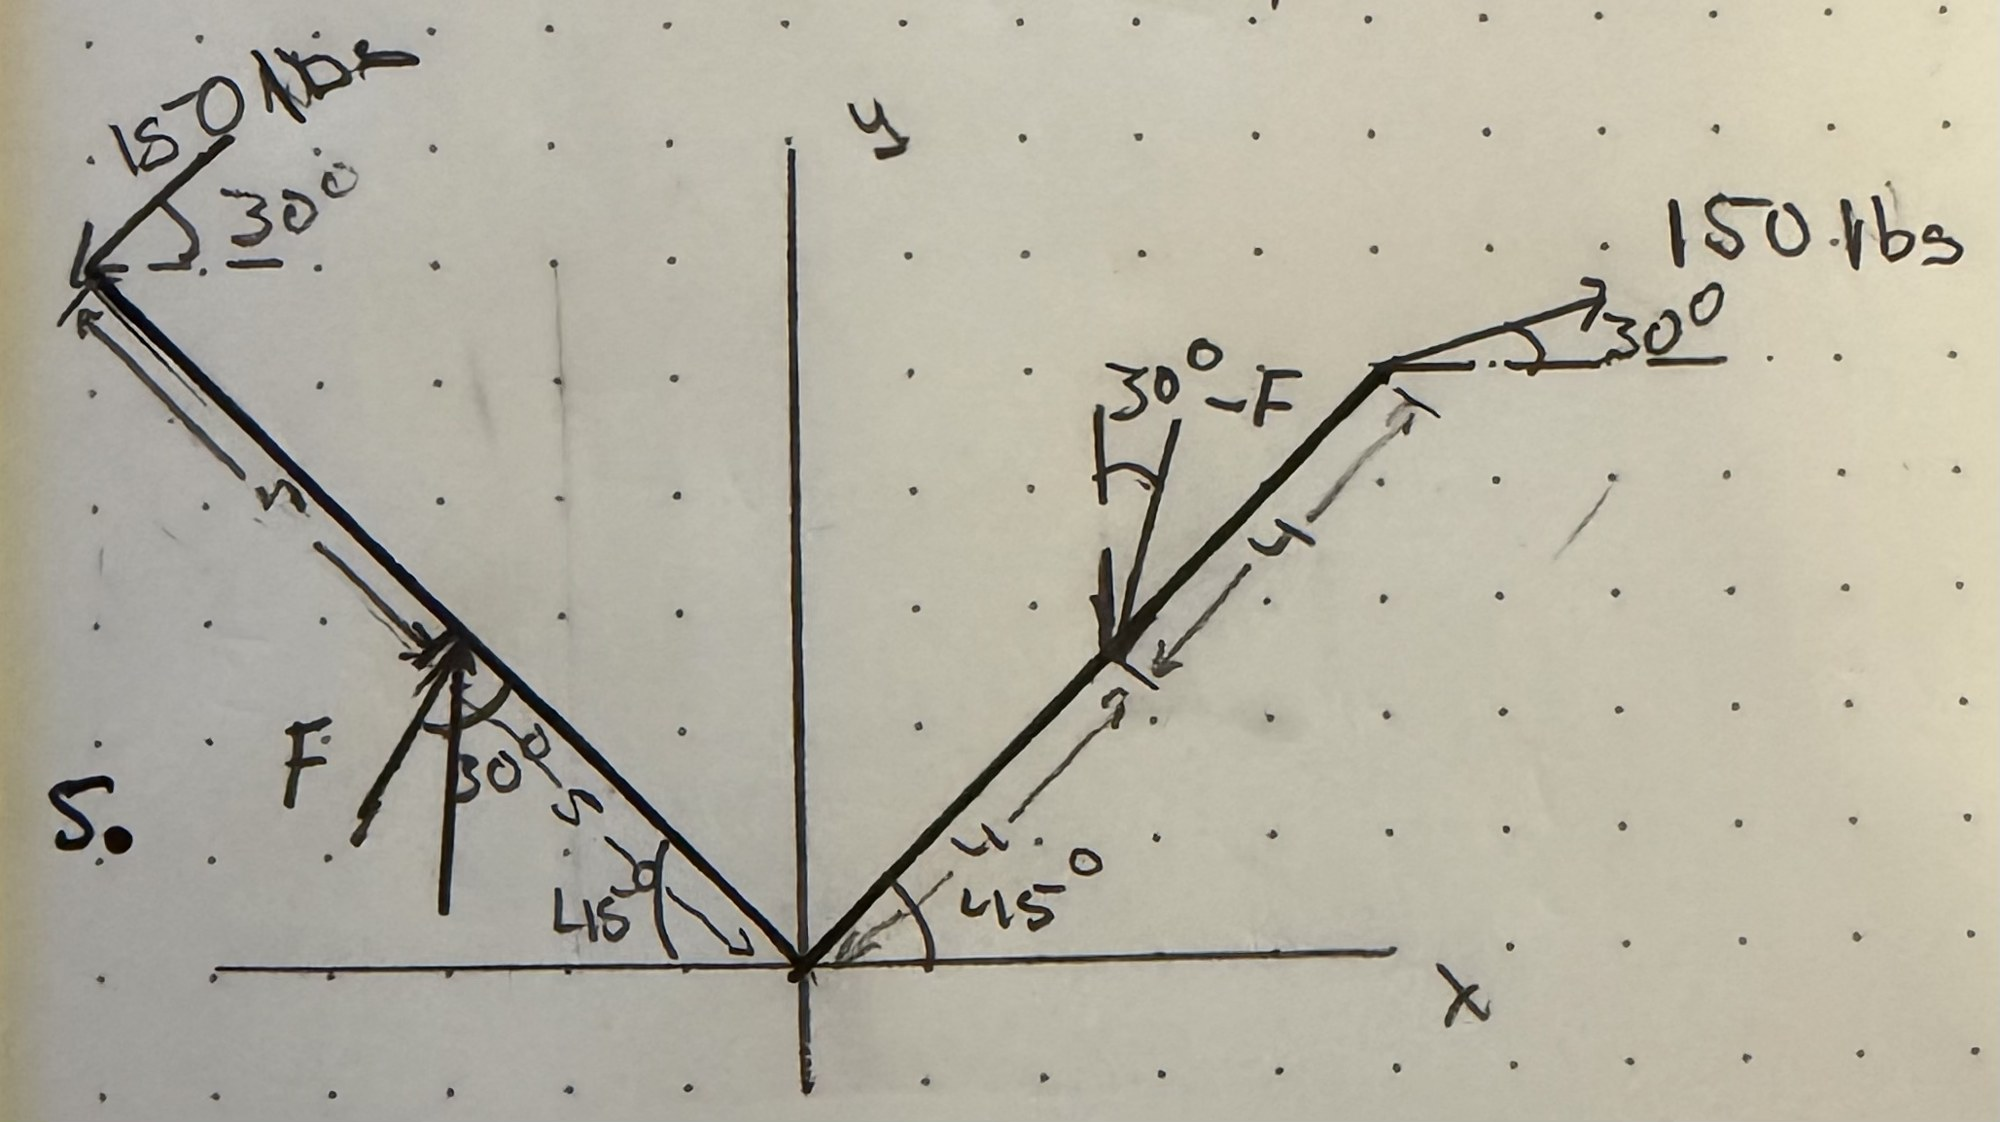
\includegraphics[width=0.7\textwidth,height=0.32\textheight,keepaspectratio]{photos/IMG_5548.jpg}
}{
Each pair of forces is equal, opposite, and parallel, so each pair is a pure couple. For a couple, $M=Fd$ with $d$ the perpendicular distance between the two lines of action, independent of the point taken.

The two pins of a pair sit symmetrically on the $45^\circ$ arms, so their separation is horizontal:
\[
s_{150}=2(9\cos45^\circ)=9\sqrt2\ \text{in},\qquad s_{F}=2(4\cos45^\circ)=4\sqrt2\ \text{in}
\]
The $150$ lb forces are $30^\circ$ from horizontal and the $F$ forces are $30^\circ$ from vertical, so
\[
d_{150}=9\sqrt2\,\sin30^\circ,\qquad d_{F}=4\sqrt2\,\cos30^\circ
\]

\textbf{Solve:} The two couples must cancel, so $150\,d_{150}=F\,d_{F}$:
\[
F=\frac{150\,(9\sqrt2\,\sin30^\circ)}{4\sqrt2\,\cos30^\circ}=\frac{1350}{4}\tan30^\circ=194.9\text{ lb}
\]
}{
$F = 195\text{ lb}$
}

\problempage{6}{
A frame is pinned at $A$. Forces act on it: $300$ N at $30^\circ$ from horizontal (0.5 m below $A$), $500$ N horizontal (1.5 m below $A$), and $400$ N vertical (0.5 m to the right, along the base). Replace this system with an equivalent resultant force and couple moment at $A$.
}{
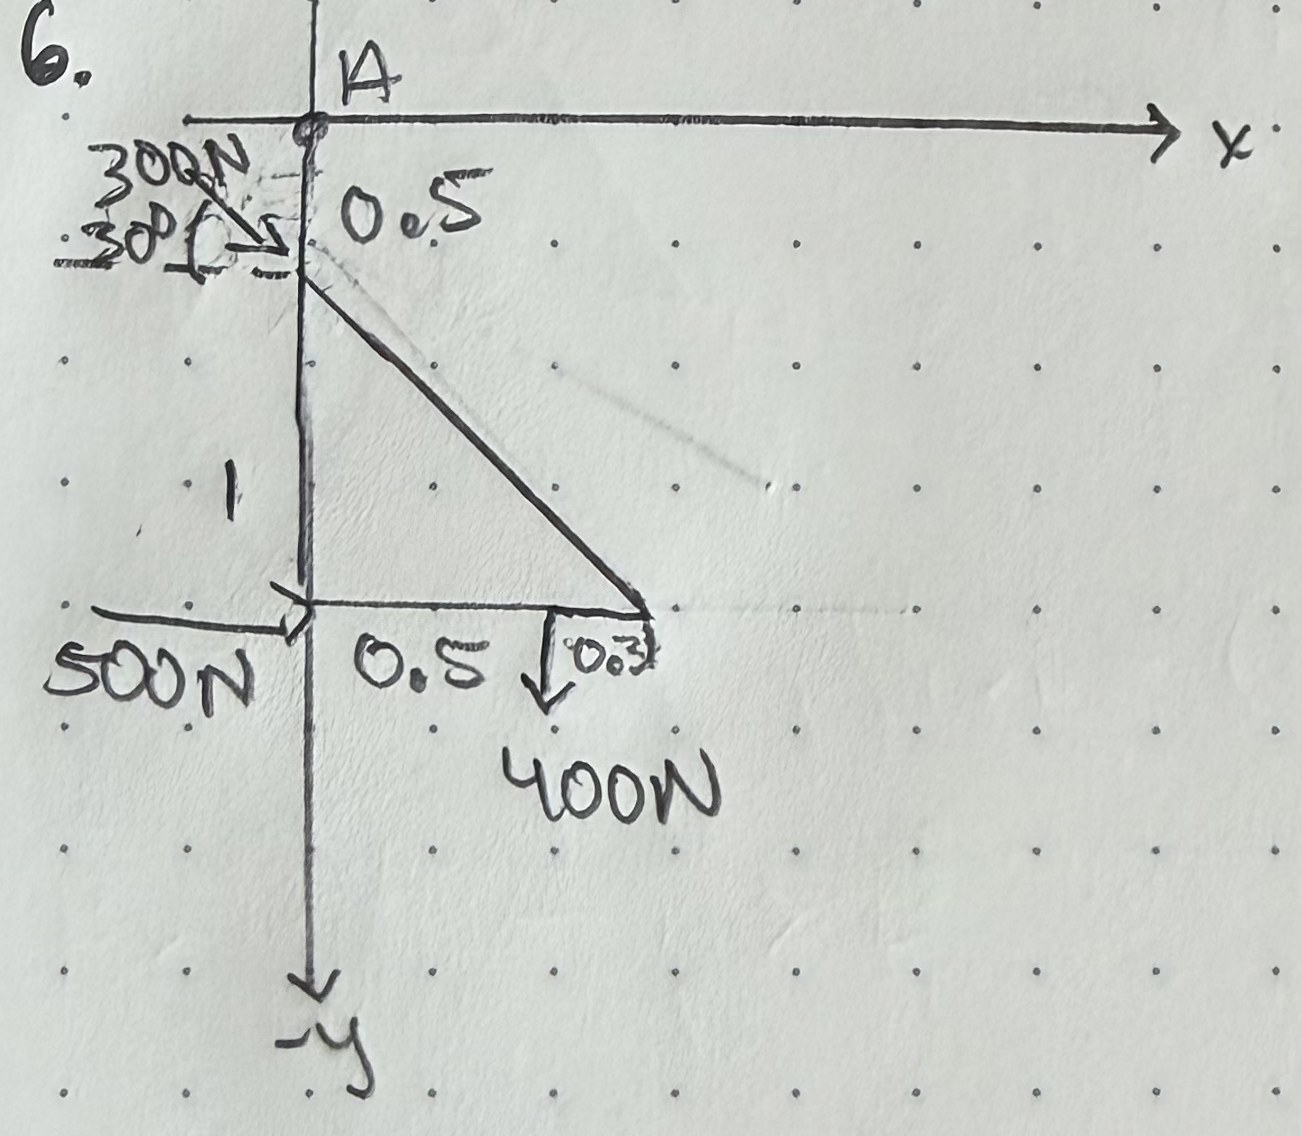
\includegraphics[width=0.7\textwidth,height=0.32\textheight,keepaspectratio]{photos/IMG_5543.jpg}
}{
Let $x$ be right, $y$ up, origin at $A$.
\[
\vec F_1 = 300(\cos30^\circ,-\sin30^\circ),\quad \vec F_2=(500,0),\quad \vec F_3=(0,-400)
\]
\[
\vec F_R=\sum\vec F_i, \qquad M_A=\sum(x_iF_{yi}-y_iF_{xi})
\]
with application points $\vec r_1=(0,-0.5)$, $\vec r_2=(0,-1.5)$, $\vec r_3=(0.5,-1.5)$ m.

\textbf{Solve:}
\[
\vec F_R = (300\cos30^\circ+500,\ -300\sin30^\circ-400) = (759.8,\ -550.0)\ \text{N}
\]
\[
|F_R|=\sqrt{759.8^2+550.0^2}=938\ \text{N}, \qquad \theta=\tan^{-1}\!\left(\frac{550.0}{759.8}\right)=35.9^\circ\ \text{below }x\text{-axis}
\]
\[
M_A = [0(-150.0)-(-0.5)(259.8)] + [0(0)-(-1.5)(500)] + [0.5(-400)-(-1.5)(0)]
\]
\[
M_A = 129.9+750.0-200.0 = 679.9\ \text{N}\cdot\text{m, CCW}
\]
}{
$F_R = 938\text{ N}$, \quad $\theta = 35.9^\circ$ below the $x$-axis, \quad $M_A = 680\text{ N}\cdot\text{m}$ (CCW)
}

\problempage{7}{
A post $AB$ (3 m tall) carries a 500 N cable (1 m below $B$, $30^\circ$ from horizontal, offset 0.2 m from centerline), a 250 N cable at $B$ (3-4-5 triangle, offset 0.5 m), and a 300 N horizontal force (2 m below $B$). Replace with a single resultant force and find where its line of action crosses post $AB$, measured from $B$.
}{
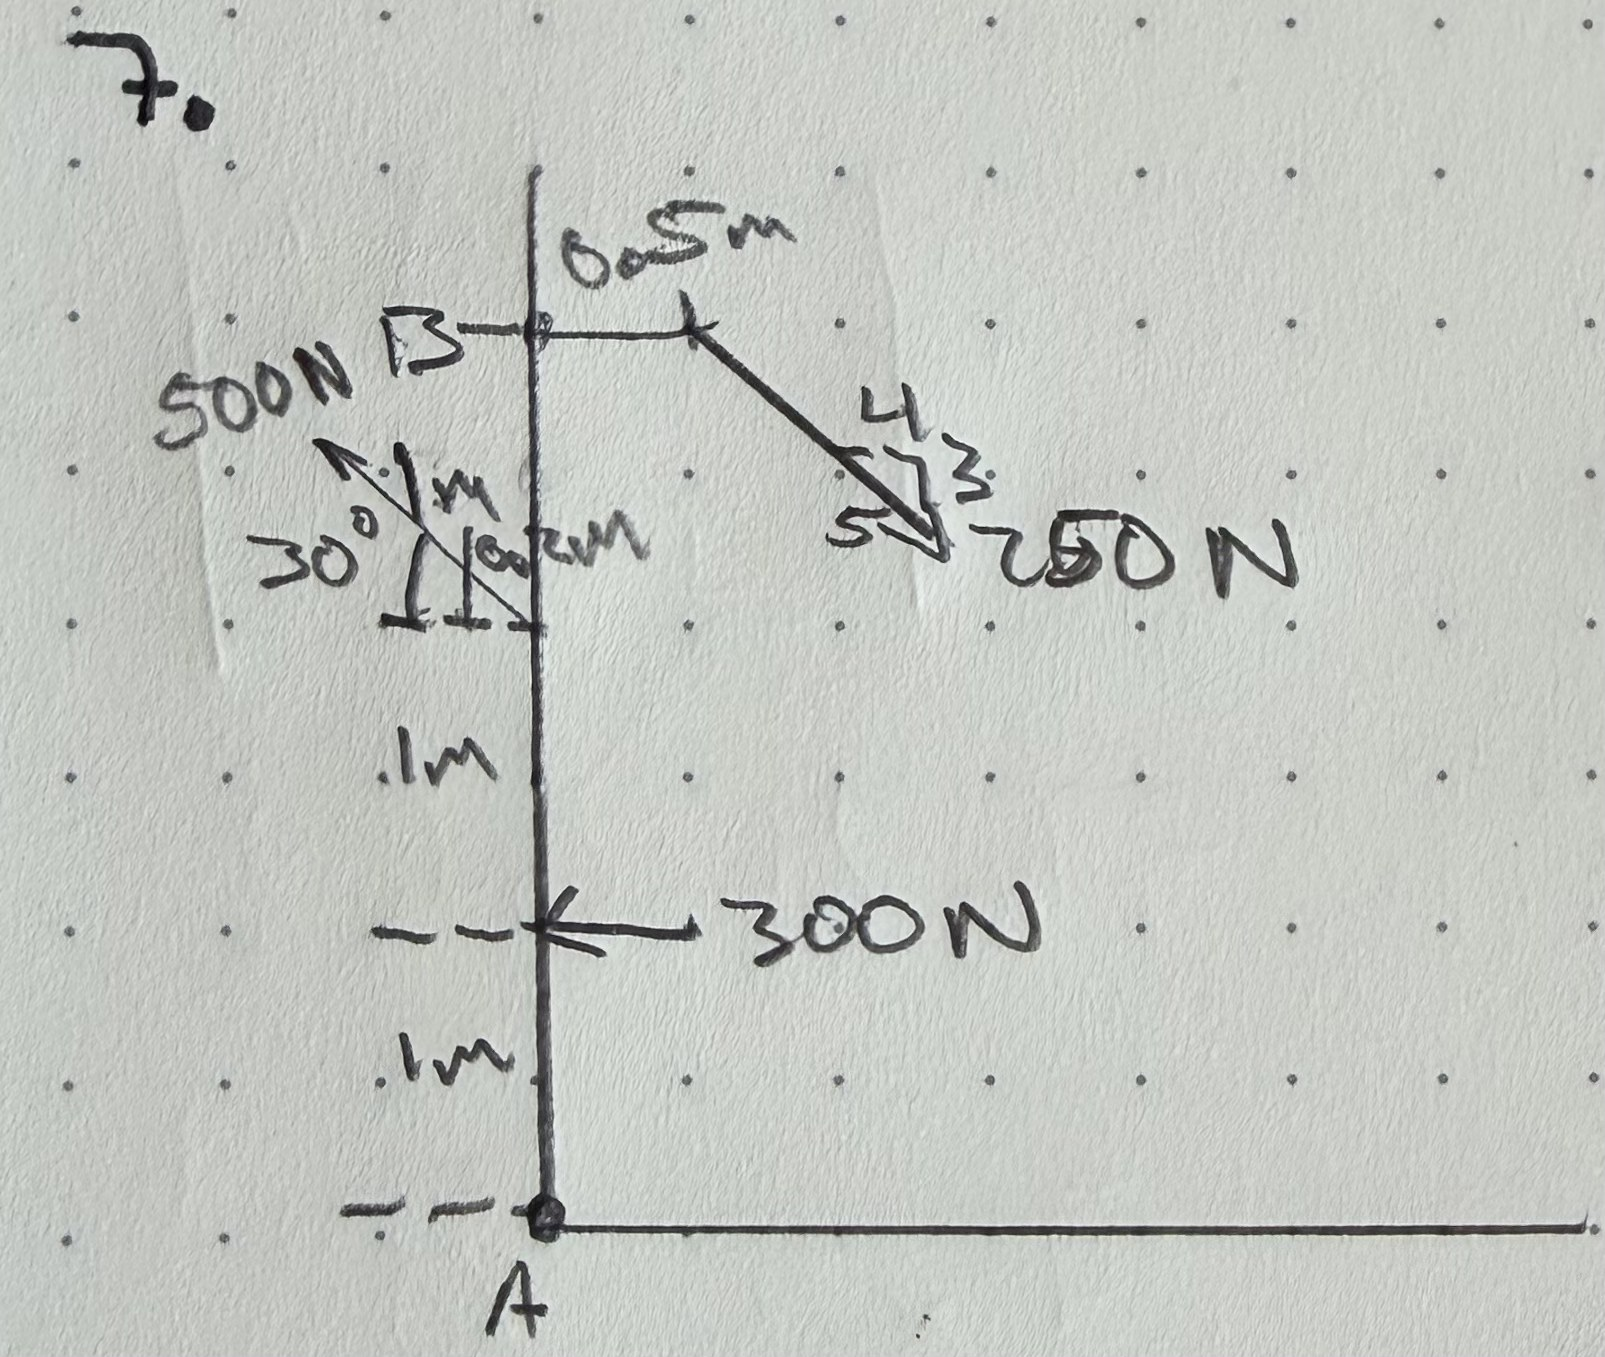
\includegraphics[width=0.7\textwidth,height=0.32\textheight,keepaspectratio]{photos/IMG_5544.jpg}
}{
With $B$ at the origin, $x$ right, $y$ up:
\[
\vec F_1=500(-\cos30^\circ,\sin30^\circ)\ \text{at } (-0.2,-1),\;
\vec F_2=250\left(\tfrac{4}{5},-\tfrac{3}{5}\right)\ \text{at } (0.5,0),\;
\vec F_3=(-300,0)\ \text{at } (0,-2)
\]
\[
\vec F_R=\sum \vec F_i, \qquad M_B=\sum (x_iF_{yi}-y_iF_{xi}), \qquad r_b = \frac{M_B}{F_{Rx}}
\]

\textbf{Solve:}
\[
\vec F_R = (-500\cos30^\circ+200-300,\ 500\sin30^\circ-150) = (-533.0,\ 100.0)\ \text{N}
\]
\[
M_B = [(-0.2)(250)-(-1)(-433.0)] + [(0.5)(-150)-0] + [0-(-2)(-300)]
\]
\[
M_B = -1158.0\ \text{N}\cdot\text{m}, \qquad r_b = \frac{-1158.0}{-533.0} = 2.17\text{ m below }B
\]
}{
$\vec F_R = -533\hat\imath+100\hat\jmath\ \text{N}$, \quad line of action crosses $AB$ at $r_b = 2.17$ m below $B$
}

\problempage{8}{
A rectangular concrete slab carries five downward point loads: $F_B=35$ kN, $F_A=40$ kN, a $30$ kN post, a $90$ kN post, and a $20$ kN post, at the $(x,y)$ locations shown. Find the resultant force and the $(x,y)$ location of its point of application.
}{
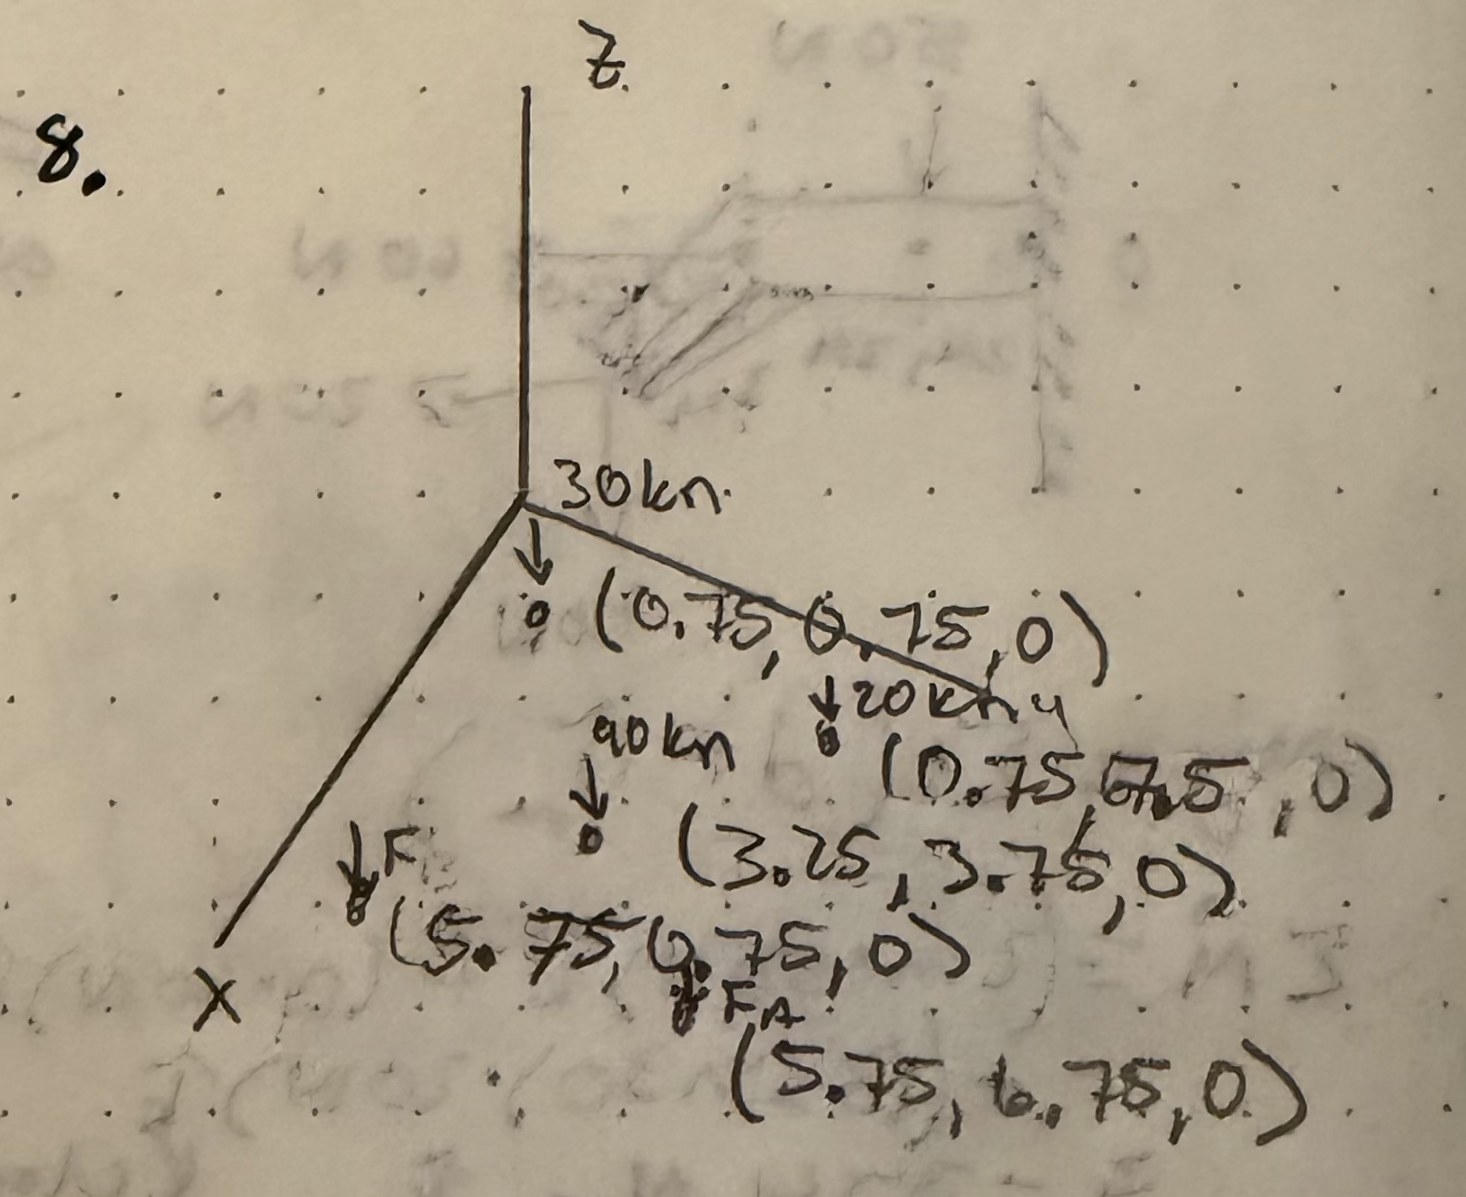
\includegraphics[width=0.7\textwidth,height=0.32\textheight,keepaspectratio]{photos/IMG_5549.jpg}
}{
All five forces are parallel (downward, $-\hat k$), so the resultant is their scalar sum, and its line of action passes through the weighted centroid of the application points:
\[
\vec F_R = -\sum F_i\,\hat k, \qquad \bar x = \frac{\sum F_i x_i}{\sum F_i}, \qquad \bar y = \frac{\sum F_i y_i}{\sum F_i}
\]
The origin is the far corner, $x$ along the $6.5$ m edge and $y$ along the $7.5$ m edge. Every post is inset $0.75$ m from its nearest edges and the center lines fall at $x=3.25$, $y=3.75$, so the loads act at $30\!:\!(0.75,0.75)$, $F_B\!:\!(5.75,0.75)$, $90\!:\!(3.25,3.75)$, $F_A\!:\!(5.75,6.75)$, $20\!:\!(0.75,6.75)$ m.

\textbf{Solve:}
\[
\sum F_i = 30+35+90+40+20 = 215\text{ kN}
\]
\[
\bar x = \frac{30(0.75)+35(5.75)+90(3.25)+40(5.75)+20(0.75)}{215}=\frac{761.25}{215}=3.54\text{ m}
\]
\[
\bar y = \frac{30(0.75)+35(0.75)+90(3.75)+40(6.75)+20(6.75)}{215}=\frac{791.25}{215}=3.68\text{ m}
\]
}{
$\vec F_R = -215\hat k\ \text{kN}$, \qquad $(x,y) = (3.54,\ 3.68)\ \text{m}$
}

\end{document}